%%%%%%%%%%%%%%%%%%%%%%%%%%%%%%%%%%%%%%%%%%%%%%%%%%%%%%%%%%%%%%%%%%%%%%%%%%%%%%%%
% \documentclass[12pt,papel,twoside]{ibtesis}
\documentclass[12pt,screen,twoside,pagebackref]{ibtesis}
% \documentclass[12pt,papel,singlespace,oneside]{ibtesis}
% \documentclass[12pt,papel,preprint,singlespace,oneside]{ibtesis}


%%%%%%%%%%%%%%%%%%%%% Paquetes extra %%%%%%%%%%%%%%%%%%%%%%%%%%%%%%%%%%%%%%%%%%%
% Por conveniencia: aqu\'{\i} puede cargar todos los paquetes y definir los %comandos que necesite
\usepackage{ibextra}
\usepackage{amsmath}
\usepackage{algorithm}
\makeatletter
\renewcommand{\ALG@name}{Algoritmo}%Cambio el titulo del entorno algoritmo por %el idioma.
\makeatother
\usepackage[noend]{algpseudocode}
\usepackage[dvipsnames]{xcolor}
%\usepackage[chapter]{algorithm}

%%%%%%%%%%%%%%%%%%%%%%%%%%%%%%%%%%%%%%%%%%%%%%%%%%%%%%%%%%%%%%%%%%%%%%%%%%%%%%%%
%%%%%%%%%%%%%%%%%%%%% Informacion sobre la tesis %%%%%%%%%%%%%%%%%%%%%%%%%%%%%%%
%\title{Titulo de la tesis}
%\author{}
%\director{}
%\codirector{}
%\carrera{Tesis Carrera de Maestr\'{\i}a en F\'isica/Ingenier'{\ia}
%\grado{Maestrando}
%\laboratorio{F\'{i}sica Estad\'{i}stica e Interdisciplinaria -- Centro At\'{o}mico Bariloche}
%\jurado{}
%\palabrasclave{}
%\keywords{}
% Si queremos poner la fecha manualmente:
%\date{Diciembre de 2099}

%%%%%%%%%%%%%%%%%%%%%%%%%%%%%%%%%%%%%%%%%%%%%%%%%%%%%%%%%%%%%%%%%%%%%%%%%%%%%%%%
%\titlepagefalse % Si no quiere compilar la portada descomente esta linea
%\includeonly{apendices} % Compilar s\'{o}lo estos archivos 
%\graphicspath{{includes/}} % Lugar donde encontrar las figuras generales (se puede poner uno en cada cap{\'{\i}}tulo)
%%%%%%%%%%%%%%%%%%%%%%%%%%%%%%%%%%%%%%%%%%%%%%%%%%%%%%%%%%%%%%%%%%%%%%%%%%%%%%%%
%\renewcommand{\i}{\italic{i}}
\begin{document}
%\maketitle
\section*{Bitácora - Maestría IB Marco Madile Hjelt- }

Este template sirve a su vez como plantilla del formato Oficial de tesis de maestría IB, cuando se descomenta lo que está comentado y se completa en los campos correspondientes tal como está indicado.\\ 

\subsection{Reunión 12 de Agosto de 2022}\\

KARINA: En esta primera reunión, Marco nos mostró la distribución de links obtenida para los encuentros en espacio y tiempo de las tortugas que veniamos monitoreando hasta ahora con tortugometro.\\
Creamos un proyecto en Github MaestriaIBMarco, donde agregué el libro de modelos para datos de telemetría de Hooten et. al. y un artículo que encontré sobre redes de interacción social de tortugas y también los nuevos datos de los 6 IgotoGPS que estuvieron monitoreando desde Enero hasta ahora.\\
Quedamos en que Marco comenzaría a hacer:\\
1) Con Igraph o networkx la matriz de adyacencia a partir de los datos. Los nodos son las tortugas y los links indican quien se encontró con quien.\\ 
2) Aumentar el grosor de links indicando cuantas veces se repitió el encuentro.\\
3) Hacer el mismo análisis con los nuevos datos de Igoto (15 días) para comparar resultados con los datos de tortugometro que están en una ventana temporal más chica (4 días).\\
4) Importante: Marco, fijate que hay una hoja que dice radiotransmisores10y30, son datos de gps medidos a mano, luego de rastrear a la tortuga con antena Yagui. Entonces seria importante verificar que esas coordenadas coinciden (dentro de cierto error) con las reportadas por en Igotu. Veo que no están ordenadas las fechas...lo que puede complicar la comparación....pero bueno hagamoslo esta vez para convencernos de que coinciden (por ejemplo yo dibujaria los puntos de tx de otro color arriba de los otros para ver si coinciden o no). Los datos de T10b.csv y T30b.csv deberían ser los mismos que los T10.csv y T30.csv de la otra carpeta.\\ 

5) Armar la red con las madrigueras nocturnas (esto lo acabo de agregar je).\\

Cosas curiosas que encontramos: la cantidad de conexiones a partir de 7 (?) sube cuando relajo el tiempo en el que cuento los eventos de encuentros espaciotemporales.\\
Adjunto un .bib pero ojo! que se que tiene muchos errores, igual sirve a modo de guía bibliográfica, no lo corrijan porque ya lo tengo corregido por ahi, luego se los paso.\\

Marco hasta reunion del 25 de agosto de 2020: \\
1) En carpeta primeras redes, arme redes de interacción de tortugas con distintas condiciones de encuentro.\\
2) agregué al codigo que el tamaño del edge sea dependiente del número de veces que  repitieron el encuentro.\\
3) agregué una función que me devuelva un dicionario de nombres de tortugas a sexo a partir de los datos guardados en csv.\\ 
4) con mismo dicionario pinte los nodos de rosa, azul y gris  para las tortugas machos, hembras y desconocidas respectivamente.\\ 
5) arme codigo para leer datos del Igoto y calcular los encuentros con este nuevo formato de archivos (excel de distintas columnas con formato variable sobre el mismo archivo).\\
6) sobre esta tarde (24/8) voy a armar las redes con estos nuevos ajustes y datos. 

\subsection*{Reunión 25 de Agosto}

KARINA, ideas para la reunión: 
0) Identificar sexo de tortugas T6, T54, T128, T184.\\
1) Identificar los refugios identificando lat, lon donde paso la noche la tortuga y dibujarlos sobre el mapa\\
2) Clasificar los "tipos de encuentros entre tortugas", si son encuentros largos (i. e., persecucion macho-
hembra o compartieron refugio por ejemplo) o si son encuentros cortos.\\ 
3) Encuentro trabajo "Inferring social structure and its drivers from refuge
use in the desert tortoise, a relatively solitary species:\\
"We show that seasonal variation has a strong impact on
tortoise burrow switching behavior.\\



4) Dos posibles papers?: \\
    a) Redes de interacción entre tortugas, estudio de las escalas temporales (igoto vs. tortugometro), 
    implicancia desde lo social y relevancia en la transmisión de enfermedades.\\
    b) Modelos de movimiento inspirados en los datos (distribucion de tamaño de paso y tiempo de espera), 
    ajustes de los modelos a los datos. Posible adaptación/extensión de los modelos de Tesis Laila para el monito? 
    por ejemplo caminatas correlacionadas (CRW). Para luego hacer el ajuste a los datos.\\

5) Pensar que tortugas conviene monitorear en la próxima campaña en funcion de estos resultados. Por ejemplo
monitorear con igoto las mismas tortugas que se han monitoreado para las redes?\\

6) Normalizar el ancho de los links (con la suma de encuentros de todos los dias de todas las tortugas (?)) para poder ver diferencia en la cantidad de encuentros durante 20min, 5 dias y 15dias
para que viendo las tres redes nos demos cuenta a simple vista de la cantidad de encuentros.

7) hacer funcion general para calcular simultaneidad en el set de datos-

%%%%%%%%%%%%%%%%%%%%%%%%%%%%%%%%%%%%%%%%%%%%%%%%%%%%%%%%%%%%%%%%%
%lo siguiente va debajo de begindocument y antes de comenzar la introduccion de la tesis.
% Dentro del environment 'preliminary' va:
% la dedicatoria, resumen, abstract, indices

%\begin{preliminary}
  
    % Escriba su dedicatoria
    %\dedicatoria{}

    %%% \'{I}ndices %%%%

   %\begin{abreviaturas}
                                %Abreviaturas
    %                                 GPU: Unidad de Procesamiento Gr\'afico %(Graphics Processing Unit)\\
    %\end{abreviaturas}
    
    %\tableofcontents                %\'{I}ndice
    
    %\listoffigures                  %Figuras
    
    %\listoftables                   %Tablas
    
    %\begin{resumen}%
    A pesar de ser una de las especies más comercializadas en el mercado ilegal de mascotas de Argentina, se conoce muy poco sobre la tortuga 
    terrestre \textit{Chelonoidis chilensis} en su hábitat natural. Debido 
    además a la creciente fragmentación de su hábitat producida principalmente 
    por la reciente introducción de ganado, esta tortuga está catalogada como 
    especie en estado 
    vulnerable. Por estos motivos resulta muy importante el 
    estudio de sus refugios, su área de movimiento y las relaciones entre 
    las tortugas dentro la comunidad. La población de estudio se encuentra 
    en el límite sur de su distribución geográfica, en las cercanías de
    San Antonio Oeste, Patagonia, Argentina. Por ser reptiles se los
    considera 
    solitarios, aunque se sabe muy poco sobre su red de interacción social. 
    En este trabajo, se estudió el movimiento de 27 individuos 
    de \textit{Chelonoidis chilensis} usando dos técnicas de monitoreo: 
    una unidad de navegación  autónoma con GPS y un \textit{datalogger} comercial. 
    Se implementó un método de filtrado de trayectorias y se construyó una 
    grilla de zonas de interés para las tortugas, utilizando las 
    trayectorias filtradas e interpoladas. Se implementaron dos criterios 
    para identificar los refugios nocturnos de las tortugas. Sobre éstos 
    se calculó la distancia media entre refugios y su centro de masa, 
    tanto para machos como para hembras y no se 
    encontraron 
    diferencias significativas en el área abarcada por los refugios para 
    ambos sexos. Se armaron redes bipartitas de nodos 
    tortuga y refugio, y se compararon las proyecciones en nodos tortuga 
    con las redes de interacción diurnas entre pares de tortugas. Se utilizó 
    la proyección en nodos tortuga de 
    la red bipartita como predictor de enlaces en la red de encuentros diurnos
    y se encontró que las predicciones no son estadísticamente significativas. 
    Se calcularon métricas sobre la topología de la red proyectada y no se 
    encontraron diferencias respecto del uso aleatorio de refugios. Finalmente
    , se descubrió la existencia de refugios preferidos y que 
    la tortuga pasa noches consecutivas en refugios geográficamente cercanos.
\end{resumen}

\begin{abstract}%
    Although it is one of the most comercialized species in the Argentinean 
    iligal
    pet market, very little is known about the \textit{Chelonoidis chilensis} 
    tortoise in the wild. This fact, together with the increasing habitat fragmentation 
    produced by cattle, that is being recently introduced into the area, lead to the 
    classification of its conservation status as vulnerable. It is therefore escencial 
    to learn about their burrows, their movement area and the relationship 
    between themselves and within their community. The studied population lives at the
    southernmost distribution of the species, near to San Antonio Oeste city in Patagonia, Argentina. 
    As they are reptiles, they are considered mostly solitary, although very little is 
    known about their social interaction network. In this work, the 
    movement of 27 \textit{Chelonoidis chilensis} tortoises were studied using two monitoring 
    techniques: an autonomous GPS navigation unit and a commercial \textit{datalogger}. A 
    trajectory filtering method was implemented and a grid was built, showing the 
    tortoises's areas of interest. Two criteria were used to identify tortoise nocturnal 
    burrows. The average distance between burrows to the center of mass 
    (of these burrows) was calculated for males and females and no significant differences
    were found. Bipartite networks of tortoise nodes and burrows were built and 
    the projection in tortoise nodes was compared with the diurnal interaction network. The 
    projection 
    in tortoise nodes of the bipartite network was used as a predictor of links 
    in the encounter diurnal network and it was found that the predictions are not 
    statistically significant. Metrics on the topology of the projected network were 
    calculated and no differences were found with respect to the random use of burrows. 
    Finally, the existence of preferred burrows was found and also that tortoises spend
    consecutive nights in nearby burrows.
\end{abstract}


%%% Local Variables: 
%%% mode: latex
%%% TeX-master: "template"
%%% End: 
 //si quiero incluir un archivo resumen.tex que esté en este mismo directorio

%\end{preliminary}

% Podemos usar cualquiera de los dos comandos: \input o \include para incluir el texto
%\chapter{Introducción}
\chapterquote{Avanza rápido el tema de las tortugas}{D. H. Zanette}
 
\section{Motivación}
El movimiento de los animales es de fundamental importancia para procesos ecológicos. Los humanos han estado interesados en el movimiento individual y poblacional por milenios. Hace más de 2000 años, Aristoteles escribió acerca del movimiento de los animales y los conceptos filosóficos y matemáticos asociados, en su libro, \textit{De Motu Animalium.} Históricamente, era crucial entender su comportamiento para saber cómo y dónde se podían obtener estas fuentes de alimento salvajes. Por lo tanto, los primeros humanos eran modeladores naturales del movimiento animal.  En tiempos modernos, estamos interesados en su movimiento por razones científicas y para poder tomar medidas de conservación y protección.
 
 
 
La mayoría de las especies animales son capaces de realizar complejos patrones de movimientos que generalmente dependen del ambiente, factores intrínsecos de los individuos y las interacciones entre ellos (\cite{morales2005adaptive}, \cite{morales2010building} y \cite{nathan2008emerging}). La complejidad de estos movimientos están manifestados en sus trayectorias. %Para el caso de las tortugas estas trayectorias dependen fuertemente de la vegetación en la zona de estudio y la época del año (caso que busquen reproducirse, depositar sus huevos, etc.).
 
 
 
\section{  \textit{Chelonoidis chilensis} }
\label{C chilensis}
 
Nuestra especie de interés es la tortuga $Chelonoidis$ $chilensis$, que se distribuye desde el Gran Chaco hasta el norte de la Patagonia, como se muestra en la Fig.~\ref{fig:distribuciondeEspecie} (\cite{chebez2008se}). Esta especie está incluida en el apéndice de la \textit{Convention on International Trade in Endangered Species of Wild Fauna and Flora (CITES)} y fue categorizada como \textit{vulnerable} a nivel nacional \cite{prado2012categorizacion} e internacional por la \textit{International Union for Conservation of Nature (IUCN)}.
Los principales factores que llevaron a esta situación son la reducción, modificación y destrucción de su hábitat, debido a la expansión de la frontera agropecuaria, así como su comercialización, siendo la especie nativa de reptiles más ilegalmente traficada en el mercado de mascotas en Argentina (\cite{prado2012categorizacion}). Además, la amenaza a esta especie se ve aumentada con la introducción de especies depredadoras exóticas como el Jabalí (\textit{Sus scrofa}) (\cite{kubisch2014chelonoidis}). En este trabajo estudiaremos una población de tortugas en en el límite sur de su distribución geográfica, a 20 km al norte de San Antonio Oeste, provincia de Río Negro, Argentina.  \\
   
Las tortugas son animales  herbívoros que se alimentan con tallos y frutos de cactus (\textit{Opuntia sulphurea, Cereus aethiops, Perocactus tuberosus}), gramíneas (\textit{Chloris castilloniana, Trhichloris crinita}), herbáceas (\textit{Alternanthera pugens, Sphaeralcea miniata, S. mendocina, Portulaca grandiflora}) y vainas de leguminosas (\cite{zacarias2016biologia}).
   
   
   
\begin{figure}[ht]
    \begin{center}
        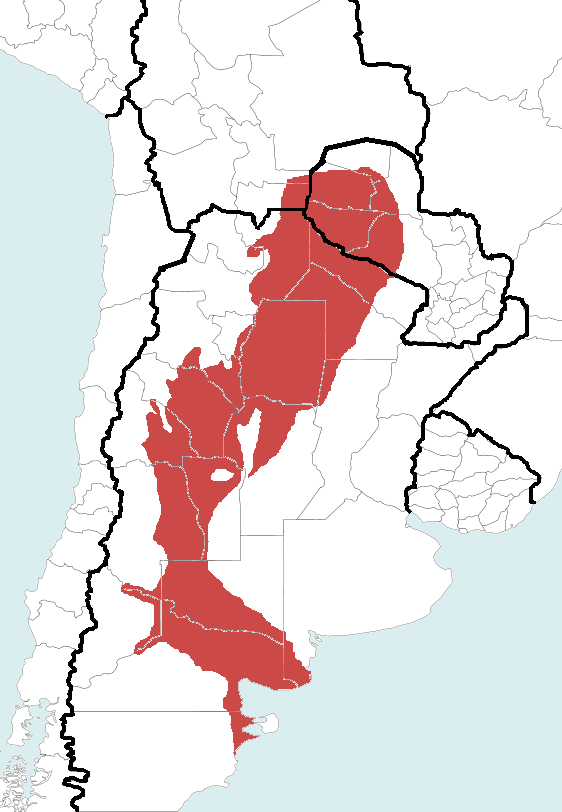
\includegraphics[width=\imsize]{figs/Chap1/Chelonoidis_chilensis_geographic_range.png}
        \caption{Distribución geográfica de la especie de tortuga \textit{Chelonoidis chilensis}
        \label{fig:distribuciondeEspecie}.}
       
        \end{center}
\end{figure}
Esta especie presenta un dimorfismo sexual cuando son adultos, siendo los machos notablemente más chicos que las hembras. El período de actividad (en la distribución más sur) de la especie a las latitudes de la zona de estudio es el más corto, ya que durante el invierno  bruman (parecido a hibernar) por aproximadamente cinco meses. Sus períodos de actividad comienzan durante la primavera, en el mes de septiembre. Desde noviembre a diciembre, ocurren los apareamientos; y entre enero y marzo es cuando las hembras pasan una gran parte del tiempo buscando un lugar adecuado para enterrar sus huevos \cite{Erika}. Al momento se conoce muy poco sobre la dinámica poblacional de C. \textit{chilensis} presente en Argentina.
 
Motivados por la falta de información, el objetivo de este estudio es caracterizar el movimiento y las interacciones de las tortugas en una de las poblaciones en el límite sur de su distribución geográfica. Aprender acerca del movimiento de los individuos es fundamental para entender su rol ecológico en el ecosistema y para diseñar políticas de conservación de la especie y su hábitat.
 
 
\section{Metodologías}
 
Se combinaron diferentes técnicas para monitorear las trayectorias de las tortugas. Para este trabajo se utilizaron datos recolectados por  el grupo de investigación (Física Estadística e Interdisciplinaria) en cuatro campañas de medición realizadas entre enero de 2020 y mayo del 2022.
 
En primer lugar se utilizó la técnica de radiotelemetría para la localización de la posición de las tortugas. En segundo lugar, se utilizó una unidad de navegación (construída en el Centro Atómico Bariloche), para registrar señales de GPS y contaba con sensores inerciales y de temperatura. En tercer lugar, más recientemente en el año 2022 se comenzó a utilizar un datalogger comercial (i-gotU GT120) que toma datos de GPS y hora. En las siguientes subsecciones se proveerán más detalles de ambas metodologías.
 
\subsection{Radiotelemetría}
La técnica de radiotelemetría permite localizar individuos mediante un sistema de transmisor-receptor-antena. Se utilizaron transmisores Holohil (Grand HOLOHIL Systems Ltd. RI-2B) pegados a los caparazones de las tortugas mediante cinta adhesiva. Estos transmisores emiten un pulso a una determinada frecuencia ($\approx$150 MHz) cada dos segundos. Los pulsos eran detectados por un sistema de recepción, que consiste en una antena Yagi-Uda conectada a un receptor ATS R410 (Advanced Telemetry Systems,Inc). Esta técnica permite con gran precisión localizar el transmisor y, usando un GPS portátil (Garmin eTrex
x20), determinar la ubicación de la tortuga.
 
A pesar de ser muy precisa espacialmente, esta técnica no posee una buena resolución temporal, necesaria para reconstruir trayectorias confiables. En primer lugar, es necesario seguir constantemente al individuo para tener una mejor resolución temporal. En segundo lugar, el investigador debe acercarse a una distancia considerable de la tortuga para tomar su posición con el GPS. Ambos factores pueden alterar el comportamiento de la tortuga y su trayectoria. En la siguiente sección se describe la unidad de navegación, que ofrece una alta resolución temporal en las trayectorias sin perturbar al comportamiento animal. Es por esta razón que solo se usó esta técnica para recuperar la unidad de navegación y el i-gotU, no para monitorear la trayectoría directamente.
 
\subsection{Unidad de navegación}
Se desarrolló en el departamento de Ingeniería del Centro Atómico  una unidad de bajo presupuesto para monitorear individuos en su hábitat natural (de ahora en más llamado tortugómetro), que consiste de un receptor GPS, sensores inerciales (acelerómetro y giróscopo) y un sensor de temperatura (Fig.~\ref{fig:tortugometro}). El mismo está alimentado por una batería recargable que le da una autonomía de aproximadamente 15 horas considerando una adquisición del GPS de un punto cada 5-10 minutos. El peso del tortugómetro es de 45 g representando el 3\% del peso de una tortuga de tamaño medio, lo que es aceptable para no disturbar el movimiento del animal. Los datos del receptor de GPS y de los sensores inerciales son guardados en una memoria micro-SD. Al final de cada día de monitoreo se descargaron los datos de la memoria y se cargaron las baterías.
 
En este trabajo, se utilizaron datos obtenidos por campañas realizadas por el grupo de investigación. Se contó con 8 de estas unidades en correcto funcionamiento para monitorear las tortugas en cada día de campaña. Las campañas de medición donde se utilizó esta técnica fueron entre enero de 2020 y enero del 2022. Se monitorearon en total 27 individuos por un total de 1160 horas.
\begin{figure}[ht]
    \begin{center}
       
   
    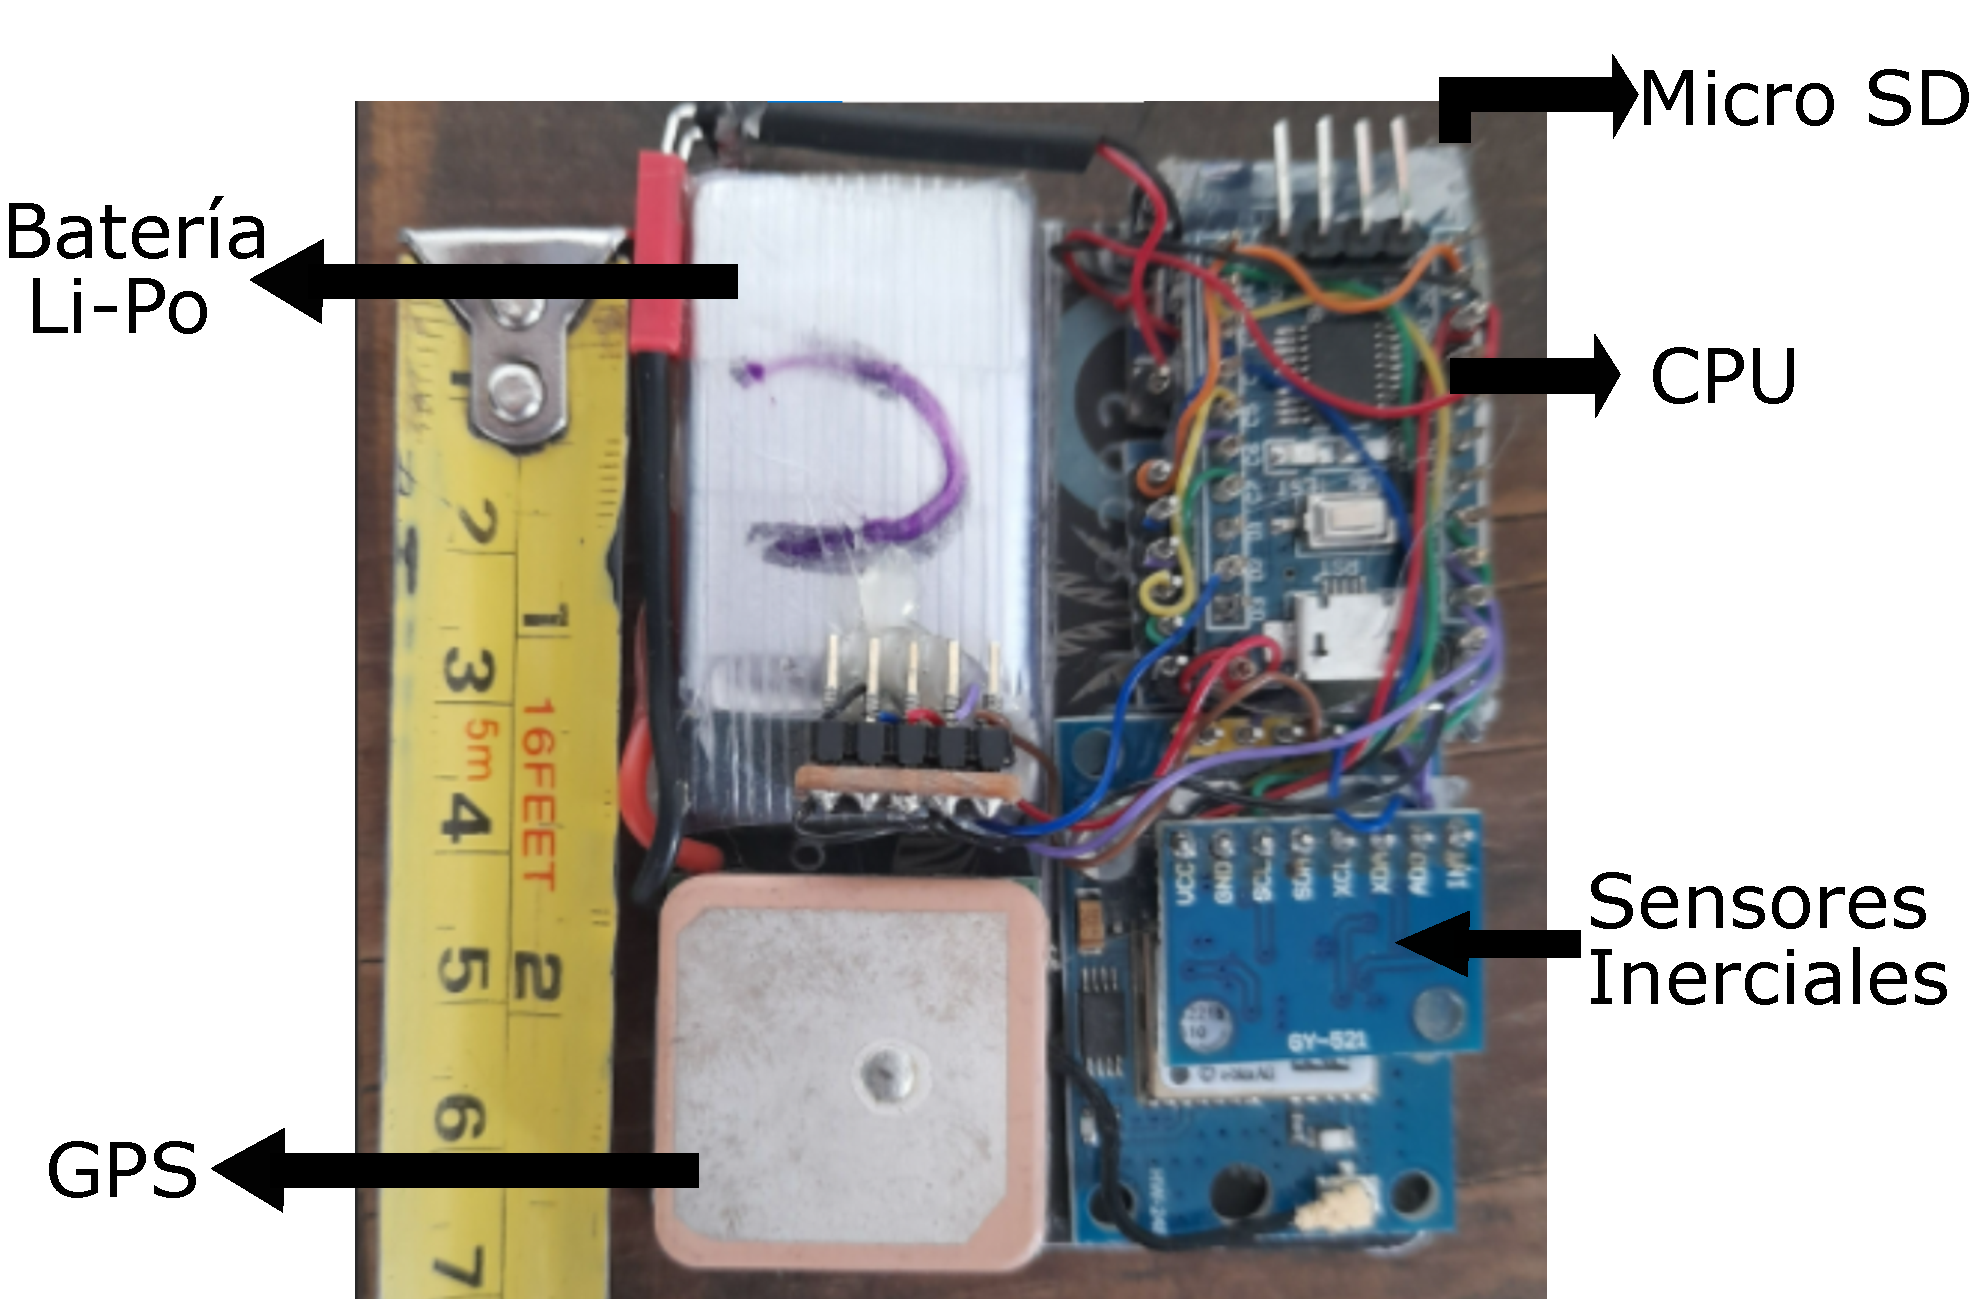
\includegraphics[width=\imsize]{figs/Chap1/tortugometro.pdf}  
\end{center}
    \caption[Unidad de navegación (tortugómetro) para monitorear individuos.] {Unidad de navegación (tortugómetro) para monitorear individuos. Consiste de un GPS, sensores inerciales (giróscopo y acelerómetro) y de temperatura, todos conectados a una unidad de control y procesamiento. Pesa menos de 45g. Las posiciones del GPS son adquiridas cada 10 minutos y se almacenan en la tarjeta micro SD extraíble. }
    \label{fig:tortugometro}
\end{figure}
 
\subsection{i-gotU}
La unidad de navegación comercial i-gotU GT120 (Fig.~\ref{fig:igotu}) es una unidad de bajo costo que permite monitorear la posición de individuos en su hábitat natural. La misma posee un receptor GPS, donde se puede programar la frecuencia de medición a través de un software provisto por el fabricante. La batería de la unidad permite una autonomía de aproximadamente 7 días. El peso de la unidad es de 21 g, lo que representa el 1.5\% del peso de una tortuga de tamaño medio. La unidad  posee una memoria interna que almacena los datos de posición y hora. Los datos se pueden descargar a la computadora a través de un puerto USB.
 
\begin{figure}[ht]
    \begin{center}
       
   
    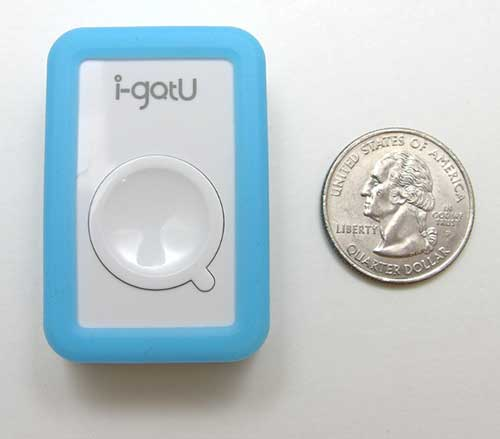
\includegraphics[width=.8\imsize]{figs/Chap1/igotu.jpg}  
\end{center}
    \caption[Unidad de navegación comercial i-gotU para monitorear individuos.] {Unidad de navegación i-gotU para monitorear individuos. Pesa aproximadamente  21\,g, las posiciones del GPS son adquiridas cada 15 minutos y se almacenan en la memoría interna del dispositivo. }
    \label{fig:igotu}
\end{figure}
Con este dispositivo se obtuvieron datos de campañas realizadas entre finales de enero 2022 y abril 2022, se contaron con 12 de estas unidades en correcto funcionamiento y se decidió monitorear a las mismas 6 tortugas intercambiando el i-gotU a cada una de ellas cada 7 días. Se programaron los i-gotU para adquirir posición y hora cada 15 minutos entre las 6 de la mañana y las 9 de la noche, sobre la noche no adquiere datos para ahorrar batería. En total se monitorearon aproximadamente 1000 horas por tortuga ya que algunas semanas no se llegó a intercambiar los i-gotU.
 
\section{Redes complejas}
El uso de herramientas de redes complejas permitió comparar resultados provenientes de diferentes análisis sobre los datos de GPS de las tortugas. En este trabajo se utilizaron métricas sobre la topología de distintas redes generadas, todas calculadas utilizando  funciones implementadas en la librería networkX de Python \cite{networkx}.
 
Una red compleja es un conjunto de elementos (nodos) conectados entre sí por enlaces (aristas). La topología de una red compleja puede ser estudiada a través de distintas métricas. En este trabajo se utilizaron las siguientes métricas:
\begin{itemize}
    \item \textbf{Densidad}: es la fracción de enlaces que existen en la red respecto de la cantidad de enlaces que podrían existir en la red. Se calcula como:
    \begin{equation}
        \rho = \frac{2m}{n(n-1)},
    \end{equation}
    donde $n$ es la cantidad de nodos y $m$ la cantidad de enlaces.
    \item  \textbf{Modularidad}: es una medida de fuerza de división de la red en comunidades. Se calcula como:
    \begin{equation}
        Q = \sum_{c=1}^{n}
        \left[ \frac{L_c}{m} - \gamma\left( \frac{k_c}{2m} \right) ^2 \right]
    \end{equation}
    donde $L_c$ es la cantidad de enlaces que conectan nodos de la comunidad $c$, $k_c$ es la cantidad de enlaces que conectan nodos de la comunidad $c$ con nodos de otras comunidades, $m$ es la cantidad de enlaces en la red y $\gamma$ es un parámetro que depende de la red. En este trabajo se utilizó $\gamma = 1$. Las comunidades en la red se identificaron a través de un método de propagación de etiquetas semi-síncrono \cite{cordasco2010community}.
    \item \textbf{Coeficiente de agrupamiento}: es una medida de la densidad de enlaces entre los vecinos de un nodo. Se calcula como:
    \begin{equation}
        c_u = \frac{2 T(u)}{deg(u)(deg(u)-1)},
    \end{equation}
    donde $T(u)$ es la cantidad de triángulos formados por los vecinos de $u$ y $deg(u)$ es la cantidad de vecinos de $u$ (grado de $u$).
 
   \item \textbf{Centralidad de grado}: para un nodo $v$, la centralidad de grado es la fracción de nodos a la que está conectado. Se calcula como:
    \begin{equation}
        C_G(v) = \frac{deg(v)}{n-1},
    \end{equation}
    donde $deg(v)$ es el grado del nodo $v$ y $n$ es la cantidad de nodos en la red. Da una idea de la importancia relativa de un nodo en la red.
 
\end{itemize}
En los siguientes capítulos se analizarán los datos obtenidos, a través de las metodologías mencionadas, mediante el enfoque de redes complejas.
 
 
 
%%% Local Variables:
%%% mode: latex
%%% TeX-master: "template"
%%% End:
 
 
 
 
 
 


%\chapter{Redes de interacción entre tortugas}
\graphicspath{{figs/}}
 
\chapterquote{In retrospect, Euler's unintended message is very simple: Graphs or networks have properties, hidden in their construction, that limit or enhance our ability to do things with them.}{Albert-László Barabási, 1982}
 
\label{Redes de interacción entre tortugas}
\section{Trayectorias }
 
En la Fig.~\ref{fig:trayeSinFiltr} se muestran las trayectorias obtenidas de los datos crudos en el día de medición 1/12/2020. Para graficar el mapa de las trayectorias se realizó un programa en el lenguaje Python utilizando la librería Folium \cite{github}.
 
\begin{figure}[ht]
    \begin{center}
       
   
    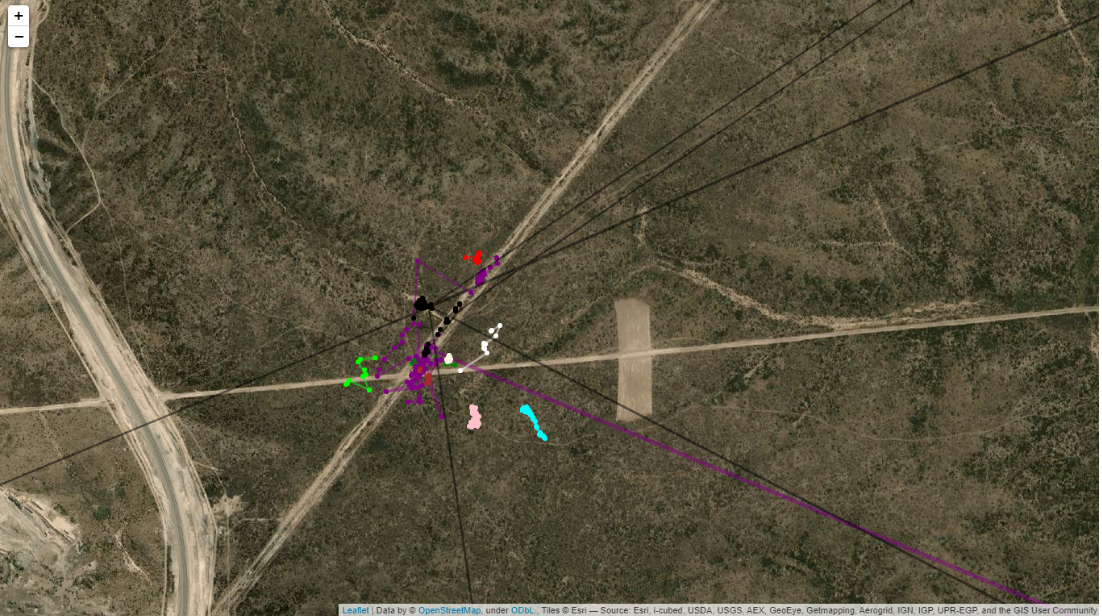
\includegraphics[width=\imsize]{Chap2/Traye1_12_sinF.png}
\end{center}
    \caption[Trayectorias un dia de medición, sin filtrar.]{Trayectorias del 1/12/2020; cada color representa una tortuga diferente. Ambas metodologías fueron implementadas; algunos puntos tomados con el tortugómetro escapan a la trayectoria esperada.}
    \label{fig:trayeSinFiltr}
\end{figure}
Se observa en la Fig.~\ref{fig:trayeSinFiltr}, que algunos puntos tomados por el tortugómetro se desvían de la trayectoria esperada para una tortuga (recorren distancias del orden de los kilómetros en menos de 10 minutos). Se estima que estas desviaciones se producen por dos motivos: en primer lugar, en los primeros minutos de medición, el GPS comienza a conectarse a satélites hasta tener la precisión máxima, haciendo que  los primeros puntos tengan una mayor desviación; en segundo lugar, se observó de manera aleatoria la desviación de algún punto respecto de la trayectoria típica. Para filtrar estas desviaciones, se implementó un método basado en la velocidad máxima que pueden alcanzar los individuos. El mismo está detallado en el repositorio de GitHub, archivo \textit{CriterioParaSacarData.py} \cite{github}. Para obtener la velocidad máxima se calculó la distribución de velocidades de la Fig.~\ref{fig:distribuciondeVel}.
 
 
\begin{figure}[ht]
\begin{center}
       
   
    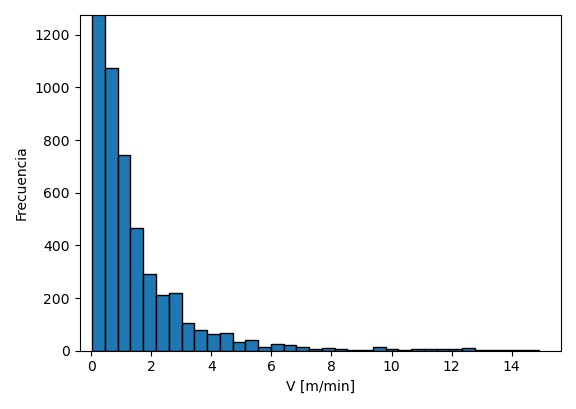
\includegraphics[width=1.2\imsize]{Chap2/Velocidades3.jpeg}
    \caption[Distribución de velocidades.]{Histograma de velocidades en m/min. Las  velocidades obtenidas mayores a 15 m/min están órdenes de magnitud por encima y fueron descartadas.}%re hacer figuras
    \label{fig:distribuciondeVel}
\end{center}
\end{figure}
Se observó en la distribución de velocidades de la Fig.~\ref{fig:distribuciondeVel}, que las tortugas llegan a una velocidad máxima de aproximadamente 15m/min, de manera que se adoptó el criterio de filtrar los tramos de trayectoria en los que la velocidad supera ese valor máximo. Filtrando los puntos de la Fig.~\ref{fig:trayeSinFiltr}, tomando velocidad máxima 15 m/min, se obtuvo  el mapa de la Fig.~\ref{fig:trayeConFiltr}.
 
 
 
 
\begin{figure}[ht]
    \begin{center}
       
   
    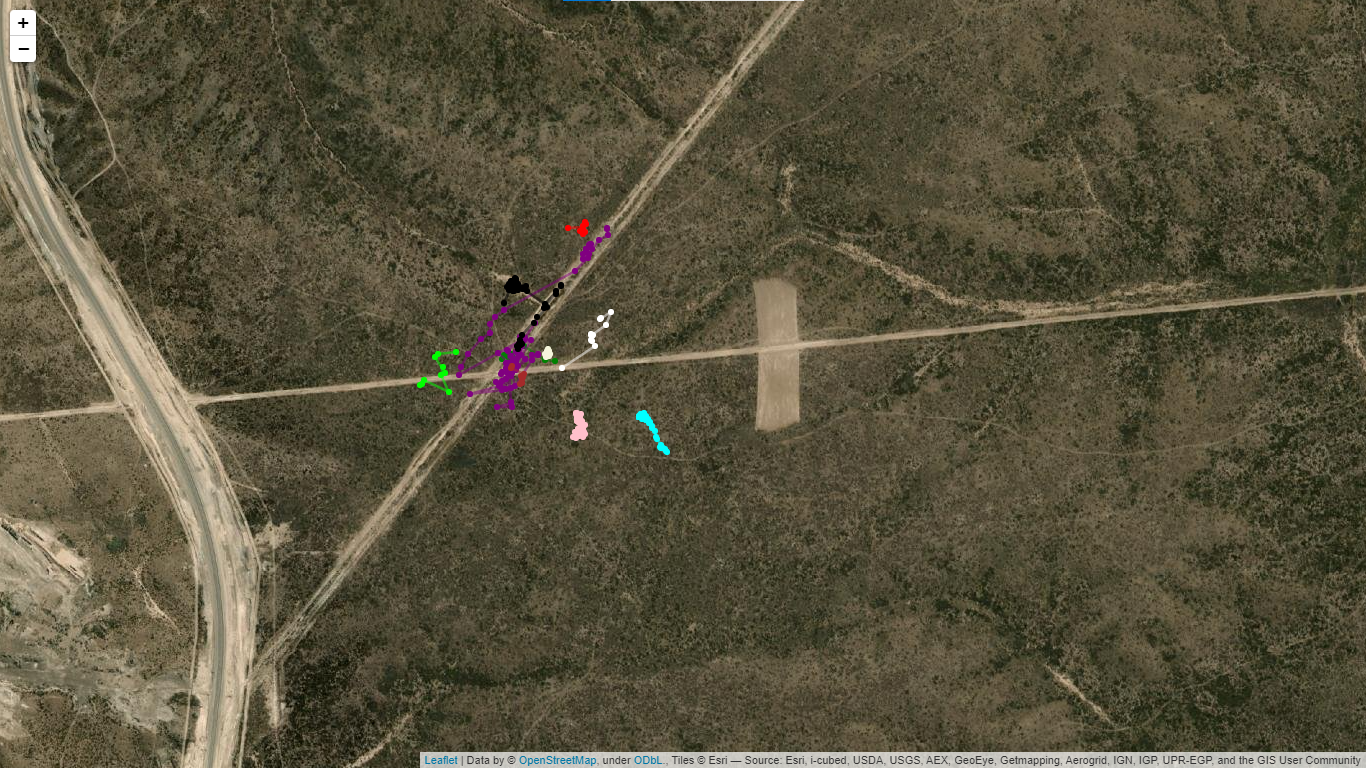
\includegraphics[width=\imsize]{Chap2/Traye1_12_conF.png}
\end{center}
    \caption[Trayectorias un dia de medición, después del filtrado.]{Trayectorias del 1/12/2020 luego del filtrado; cada color representa una tortuga diferente.}
    \label{fig:trayeConFiltr}
\end{figure}
 
\section{Zonas de interés}
Partiendo de las trayectorias filtradas, se realizó  una grilla identificando las zonas de recurrencia en la Fig.~\ref{fig:grilla1}. Las celdas de la grilla fueron elegidas de 10\,m$^2$ debido a que se estima en 10\,m el erorr del GPS del tortugómetro. Para cada celda se contó el numero de veces que estuvo allí, la grilla fue programada en Python \cite{github}. En caso de que se pudieran identificar los factores o características de las zonas más recurridas, se podrían sugerir políticas de manejo para minimizar los daños sobre las tortugas. Esto es especialmente importante dado que ahora se está introduciendo ganado en la zona con el consiguiente deterioro del hábitat natural de las mismas.
 
 
\begin{figure}[ht]
    \begin{center}
    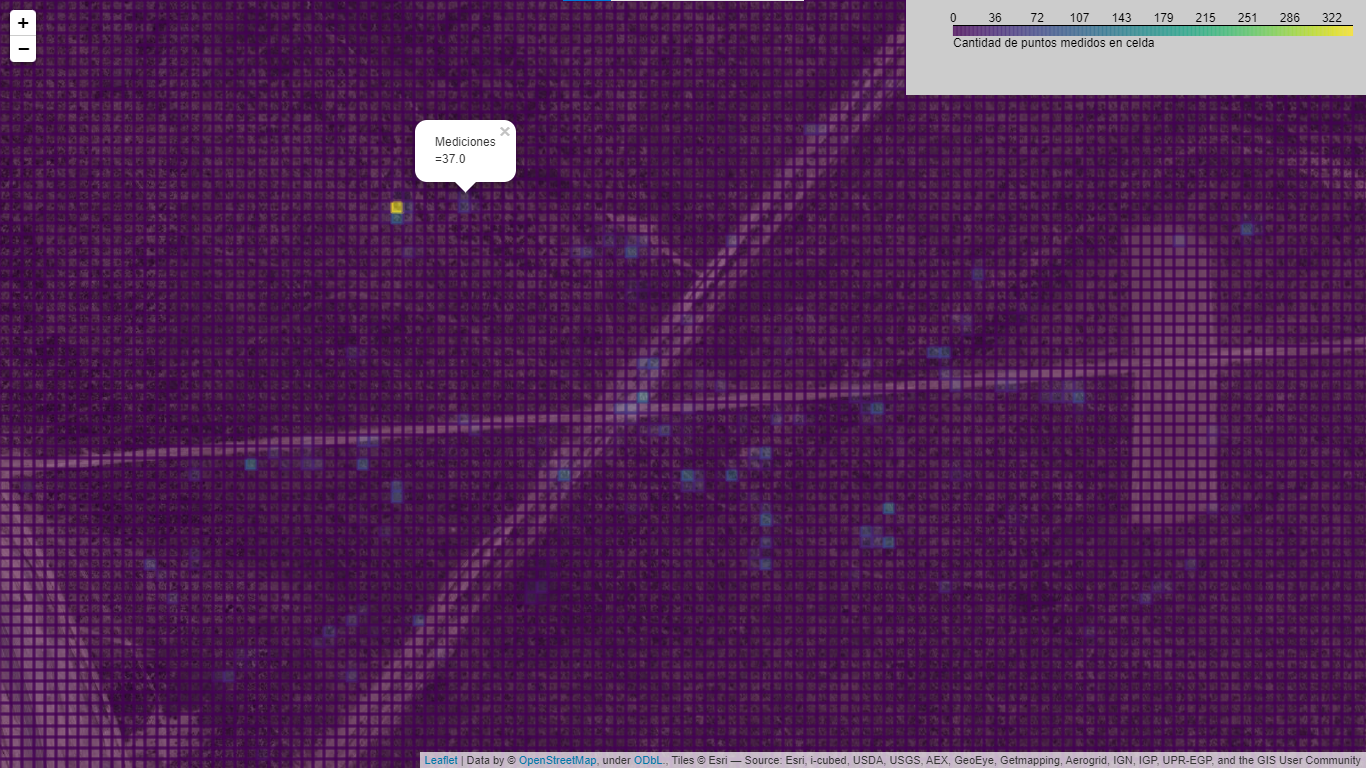
\includegraphics[width=\imsize]{Chap2/GrillaSintCNoche.png}
    \end{center}
    \caption[Mapa de zonas de recurrencia.]{Mapa de recurrencias  interactivo con las trayectorias filtradas. Al hacer clic en cualquier celda de la grilla un cartel dice cuantas mediciones fueron tomadas. El tamaño de celda es de 10m$^2$.}
    \label{fig:grilla1}
\end{figure}
 
Se puede observar en la Fig.~\ref{fig:grilla1} un punto que se destaca mucho más que el resto (arriba a la izquierda) teniendo el máximo de mediciones en esa casilla. Esto se debe a que una pareja de tortugas pasó la noche con el tortugómetro puesto en medio de un arbusto de difícil acceso. Para obtener una mejor idea de las zonas de interés diurnas se realizó otra grilla usando sólo datos del tortugómetro registrados en el día (entre 7am y 9pm) y  realizando una interpolación lineal de 1 punto por minuto por cada par de puntos consecutivos (Fig.~\ref{fig:grillaInt}, \cite{github}). Esta interpolación da una aproximación de las casillas por donde tuvo que pasar la tortuga y añade un peso cuando la tortuga se quedó dentro de la misma casilla por una mayor cantidad de tiempo (mediciones consecutivas).
 
\begin{figure}[ht]
    \begin{center}
       
   
    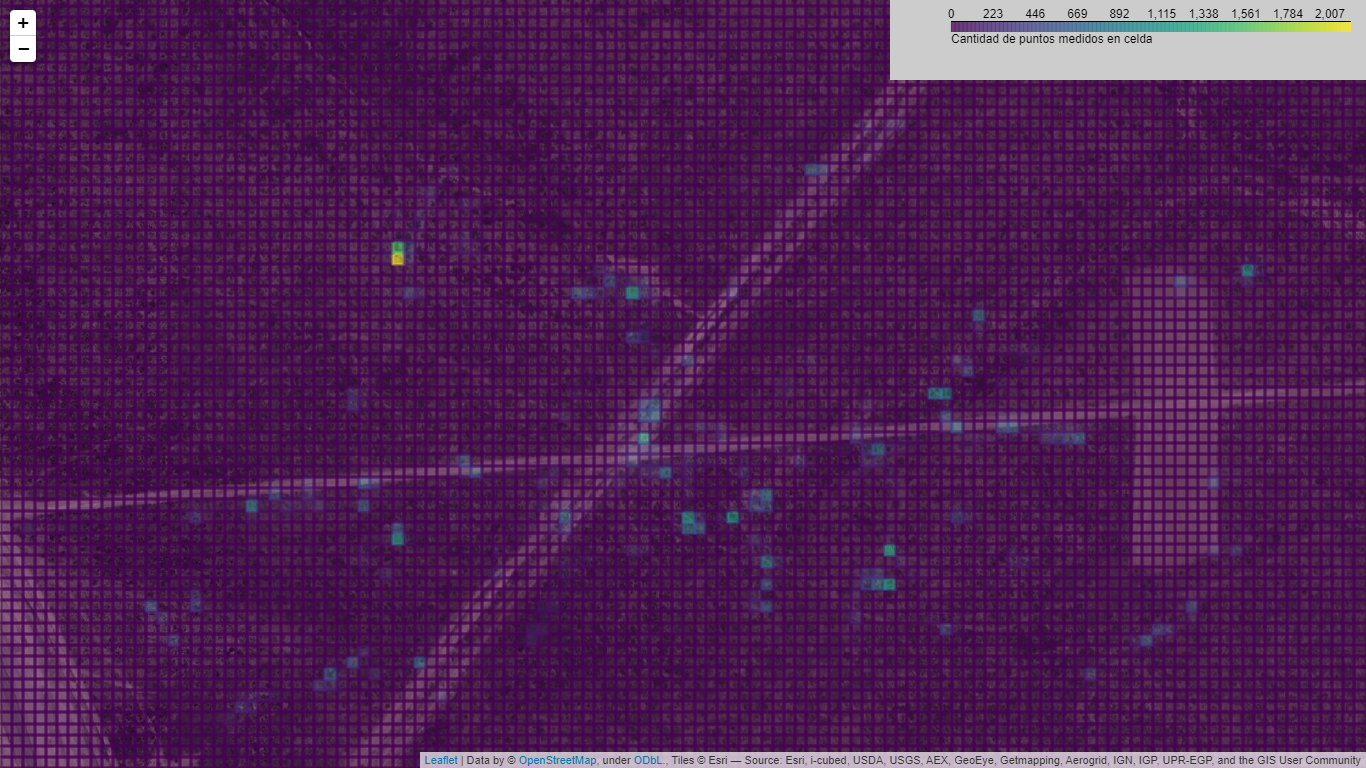
\includegraphics[width=\imsize]{Chap2/GrillaCintSNoche.png}
\end{center}
    \caption[Mapa con zona de recurrencia para trayectorias diurnas.]{Mapa de recurrencias  interactivo con las trayectorias diurnas (7am-9pm) filtradas e interpoladas linealmente. Al hacer clic en cualquier celda de la grilla un cartel dice cuantas mediciones fueron tomadas. El tamaño de celda es de 10m$^2$.}
    \label{fig:grillaInt}
\end{figure}


Comparando las Figs. \ref{fig:grilla1} y \ref{fig:grilla1}, se observa en la  Fig.~\ref{fig:grillaInt} un mayor contraste de las otras celdas respecto al que se encuentra arriba a la izquierda. Esto se debe a la extracción de los puntos nocturnos. Al momento se desconocen los motivos por los cuales dichas zonas son muy visitadas, esto será investigado en profundidad en el futuro.
 
\section{Red de encuentros}
Partiendo de las trayectorias filtradas, se decidió buscar el solapamiento de las trayectorias, para identificar los encuentros. Para ello, se implementó un código en Python que, partiendo de cualquier punto de su trayectoria, busca si hay otro punto de otra tortuga que se encuentre a una distancia menor a 20 metros y a una distancia temporal menor a 20 minutos. Cuando se cumple esta condición se van guardando los pares de puntos junto con la hora y el nombre de ambas tortugas.
 
En las Figs. \ref{fig:encuentros_hora_medida_tortugometro} y \ref{fig:encuentros_hora_medida_igotu}, pueden verse la cantidad de encuentros calculados por hora medida por los tortugómetros y por los i-gotU en función de los meses de medición. Los encuentros del tipo macho-hembra fueron normalizados por la cantidad promedio de horas medidas de ambos sexos para cada mes, en cambio para la cantidad de encuentros macho-macho y hembra-hembra se normalizó utilizando la cantidad de horas medidas para cada sexo en cada mes.  
\begin{figure}[ht]
    \begin{center}
       
   
    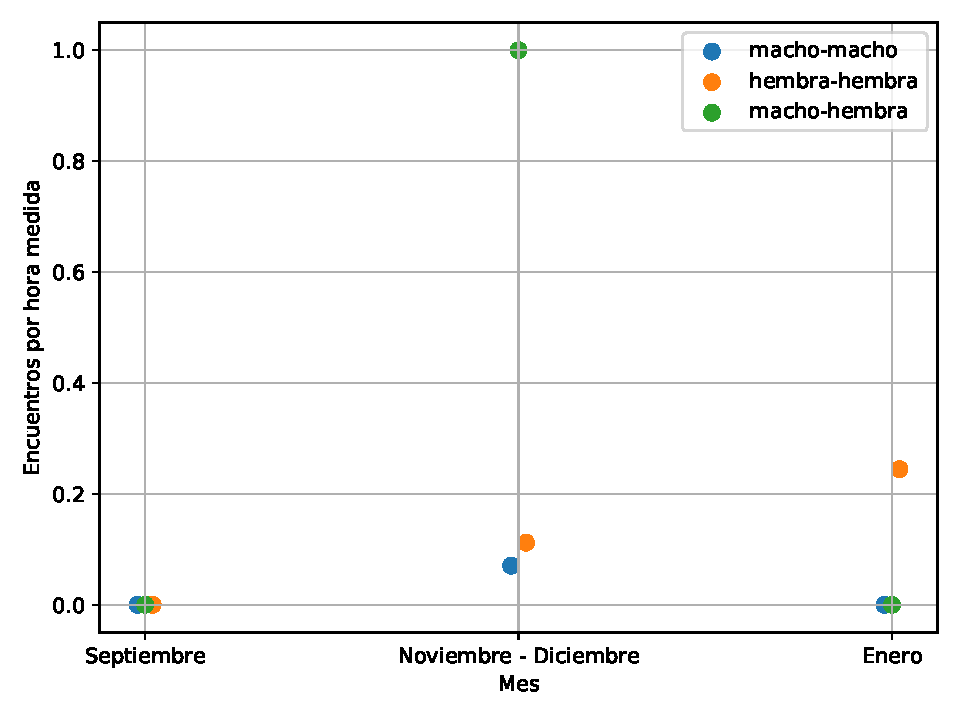
\includegraphics[width=\imsize]{Chap2/encuentros_por_hora_tortugometro.pdf}
\end{center}
    \caption[Encuentros por hora medida tomando los datos del tortugómetro.]{Encuentros sobre cantidad de horas medidas para cada sexo en función de los meses de medición utilizando el tortugómetro. Los distintos colores identifican el tipo de encuentro.}
    \label{fig:encuentros_hora_medida_tortugometro}
\end{figure}
 
\begin{figure}[ht]
    \begin{center}
       
   
    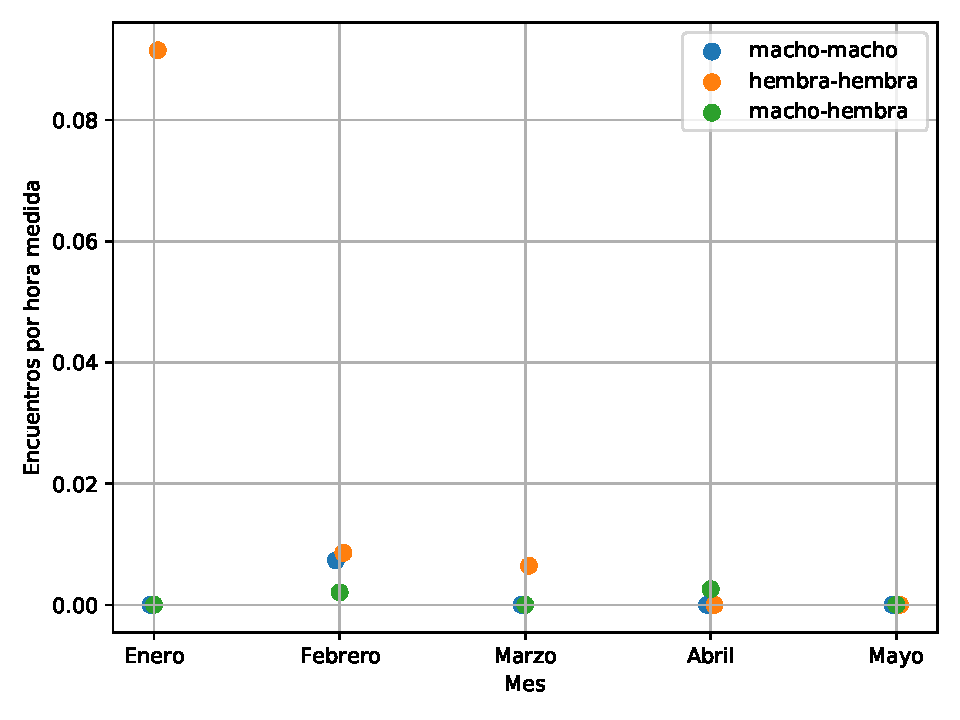
\includegraphics[width=\imsize]{Chap2/encuentros_por_hora_igotu.pdf}
\end{center}
    \caption[Encuentros por hora medida tomando los datos de los i-gotU.]{Encuentros sobre cantidad de horas medidas para cada sexo en función de los meses de medición utilizando los i-gotU. Los distintos colores identifican el tipo de encuentro.}
    \label{fig:encuentros_hora_medida_igotu}
\end{figure}
En la Fig. \ref{fig:encuentros_hora_medida_tortugometro}, se observa que el máximo de encuentros del tipo macho-hembra por hora medida ocurre en los meses noviembre-diciembre; esto coincide con la época de apareamiento. Estos meses están juntos ya que las mediciones en esos meses fueron tomadas a finales de noviembre y principios de diciembre. Para el mes de enero solo se registraron encuentros del tipo hembra-hembra en ambas figuras ( \ref{fig:encuentros_hora_medida_tortugometro} y \ref{fig:encuentros_hora_medida_igotu}), esto puede deberse a que las hembras están buscando un lugar acorde para depositar sus huevos, haciendo el encuentro hembra-hembra más probable. Para los datos de los i-gotU (\ref{fig:encuentros_hora_medida_igotu}) también se registraron encuentros en los meses de febrero, marzo y abril, pero en menor cantidad que en los meses anteriores, asociamos esta diferencia a la disminución de actividad en las tortugas propia de este periodo.
 
 
Utilizando los encuentros calculados, se armaron dos redes de interacción  utilizando la librería NetworkX \cite{networkx}, una para los datos obtenidos con  tortugómetro y otra para los datos provenientes de i-gotU (Figs. \ref{fig:redInteraccion20mincampanas} y \ref{fig:redInteraccion20igotu}). Las conexiones entre nodos tortugas tienen peso linealmente dependiente de la cantidad de encuentros entre ellas, esto se observa en el grosor del link entre dos tortugas y las distancias relativas entre nodos.
 
 
\begin{figure}[ht]
    \begin{center}
       
   
    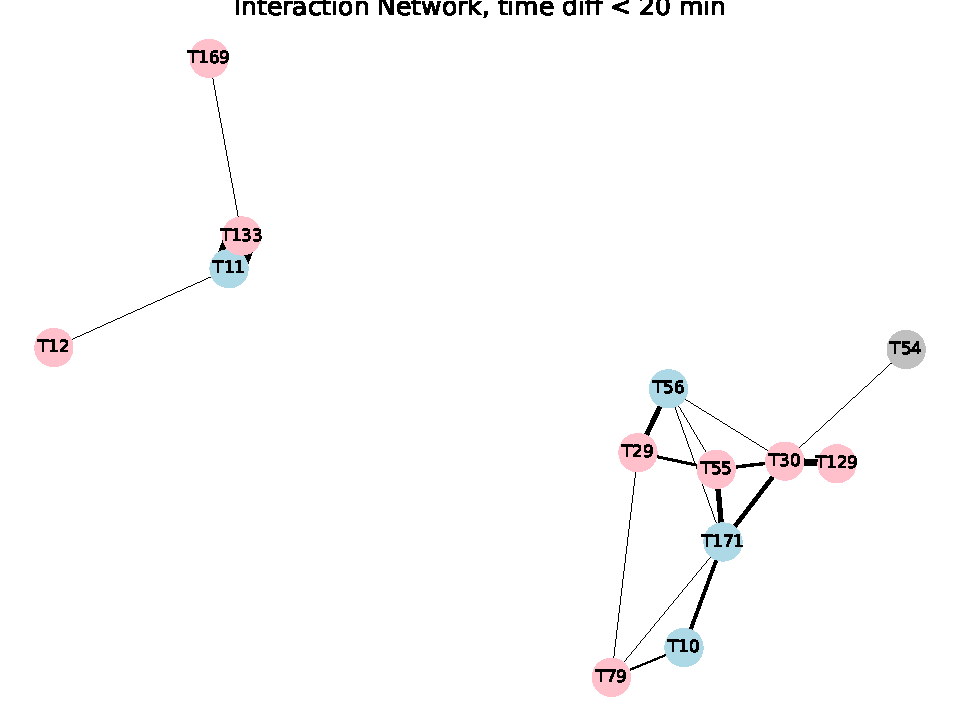
\includegraphics[width=\imsize]{Chap2/red_interaccion_20min_campanas.pdf}
\end{center}
    \caption[Red de encuentros entre tortugas  con datos tomados por el tortugómetro.]{Red de encuentros entre tortugas para datos provenientes de la metodología  tortugómetro. La condición de encuentro está dada por una distancia espacial menor a 20 metros y a una distancia temporal menor a 20 minutos. Los datos de tortugómetros fueron tomados en distintas campañas en los meses de octubre, noviembre, diciembre y mediados de enero.}
    \label{fig:redInteraccion20mincampanas}
\end{figure}
 
 
 
\begin{figure}[ht]
    \begin{center}
       
   
    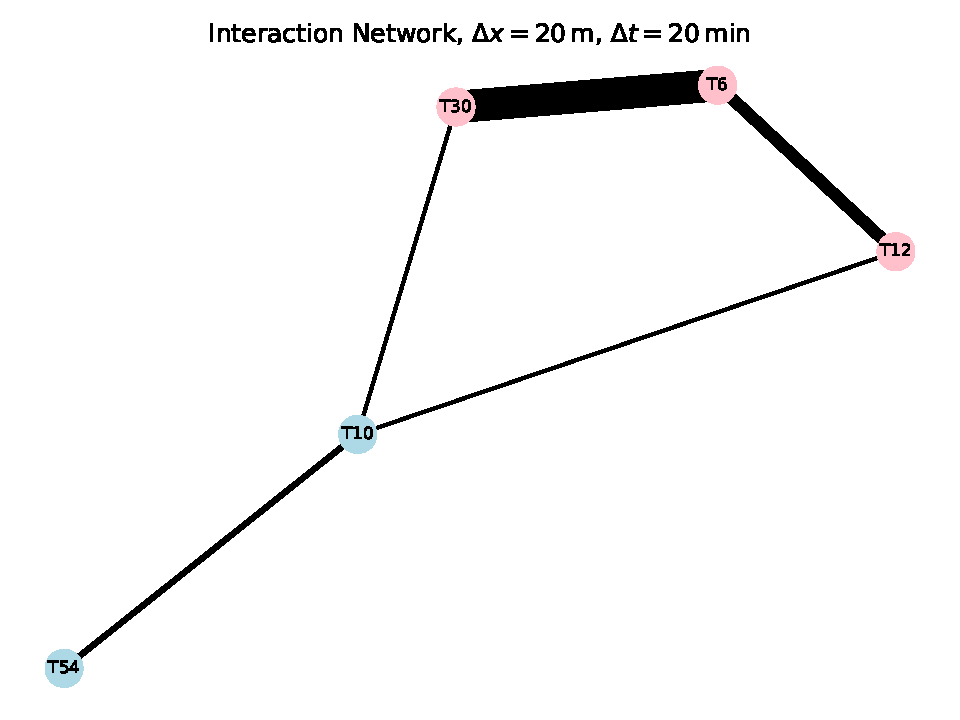
\includegraphics[width=\imsize]{Chap2/red_interaccion_20min_IGOTO.pdf}
\end{center}
    \caption[Red de encuentros entre tortugas utilizando i-gotU.]{Red de encuentros entre tortugas para datos provenientes de las metodologías i-gotU. La condición de encuentro está dada por una distancia espacial menor a 20 metros y a una distancia temporal menor a 20 minutos. Los datos de los i-gotU fueron tomados desde finales de febrero hasta principios de mayo.}
    \label{fig:redInteraccion20igotu}
\end{figure}
 
 
En la Fig. \ref{fig:redInteraccion20mincampanas}, se observa que la red de interacción está compuesta por dos comunidades. Sobre estas comunidades, se calcularon la media de las posiciones de cada nodo tortuga junto con su desviación estándar y no se encontraron diferencias significativas en estos valores para  nodos tortugas pertenecientes a cada una de las comunidades. Esto nos indica que las tortugas que pertenecen a cada comunidad, no están separadas en el espacio y no es la causa de la separación de la red en dos comunidades. Queda a determinar en futuros trabajos si la separación de la red en estas dos comunidades está relacionada con la cantidad de  mediciones o con alguna característica de la población de tortugas estudiada. En la red, también se observan diferencias  de grado, teniendo algunas tortugas muchas más conexiones que otras. Se seguirá trabajando para identificar comportamientos particulares de las tortugas que puedan estar relacionados con la distribución de grado de la red.
 
En la Fig. \ref{fig:redInteraccion20igotu}, se observa una mayor cantidad de encuentros entre las tortugas hembras (grosor de enlace), esto puede deberse a la época de medición, ya que en enero las tortugas hembras están en búsqueda de algún lugar para depositar sus huevos. En el siguiente capítulo se analizarán redes bipartitas de refugios y se compararan con las redes de interacción de tortugas para entender mejor este aspecto.
 
%%% Local Variables:
%%% mode: latex
%%% TeX-master: "template"
%%% End:
 
 
 



%\appendix
%\chapter{Ejemplo de ap\'{e}ndice: El problema de la medida \LGM{sacar/modificar}}\label{C:ap1}
\chapterquote{Negociemos Don Inodoro}{Fernando de la R\'{u}a, 2001}
\chapterquote{Smartness runs in my family.  When I went to school I was so smart my
teacher was in my class for five years}{George Burns}
\graphicspath{{figs/}}
%%%%%%%%%%%%%%%%%%%%%%%%%%%%%%%%%%%%%%%%%%%%%%%%%%%%%%%%%%%%%%%%%%%%%%%%
El gran problema lo constituye el proceso de medici\'{o}n. En la f\'{\i}sica cl\'{a}sica, medir significa revelar o poner de manifiesto propiedades que estaban en el sistema desde antes de que midamos \cite{Philipp1982NCBSp75}.

En mec\'{a}nica cu\'{a}ntica el proceso de medici\'{o}n altera de forma incontrolada la evoluci\'{o}n del sistema. Constituye un error pensar dentro del marco de la f\'{\i}sica cu\'{a}ntica que medir es revelar propiedades que estaban en el sistema con anterioridad. La informaci\'{o}n que nos proporciona la funci\'{o}n de onda es la distribuci\'{o}n de probabilidades, con la cual se podr\'{a} medir tal valor de tal cantidad. Cuando medimos ponemos en marcha un proceso que es indeterminable a priori, lo que algunos denominan azar, ya que habr\'{a} distintas probabilidades de medir distintos resultados. Esta idea fue y es a\'{u}n objeto de controversias y disputas entre los f\'{\i}sicos, fil\'{o}sofos y epistem\'{o}logos. Uno de los grandes objetores de esta interpretaci\'{o}n fue Albert Einstein, quien a prop\'{o}sito de esta idea dijo su famosa frase "Dios no juega a los dados".

Independientemente de los problemas de interpretaci\'{o}n, la mec\'{a}nica cu\'{a}ntica ha podido explicar esencialmente todo el mundo microsc\'{o}pico y ha hecho predicciones que han sido probadas experimentalmente de forma exitosa, por lo que es una teor\'{\i}a un\'{a}nimemente aceptada.

\begin{figure}[ht]
\centering{}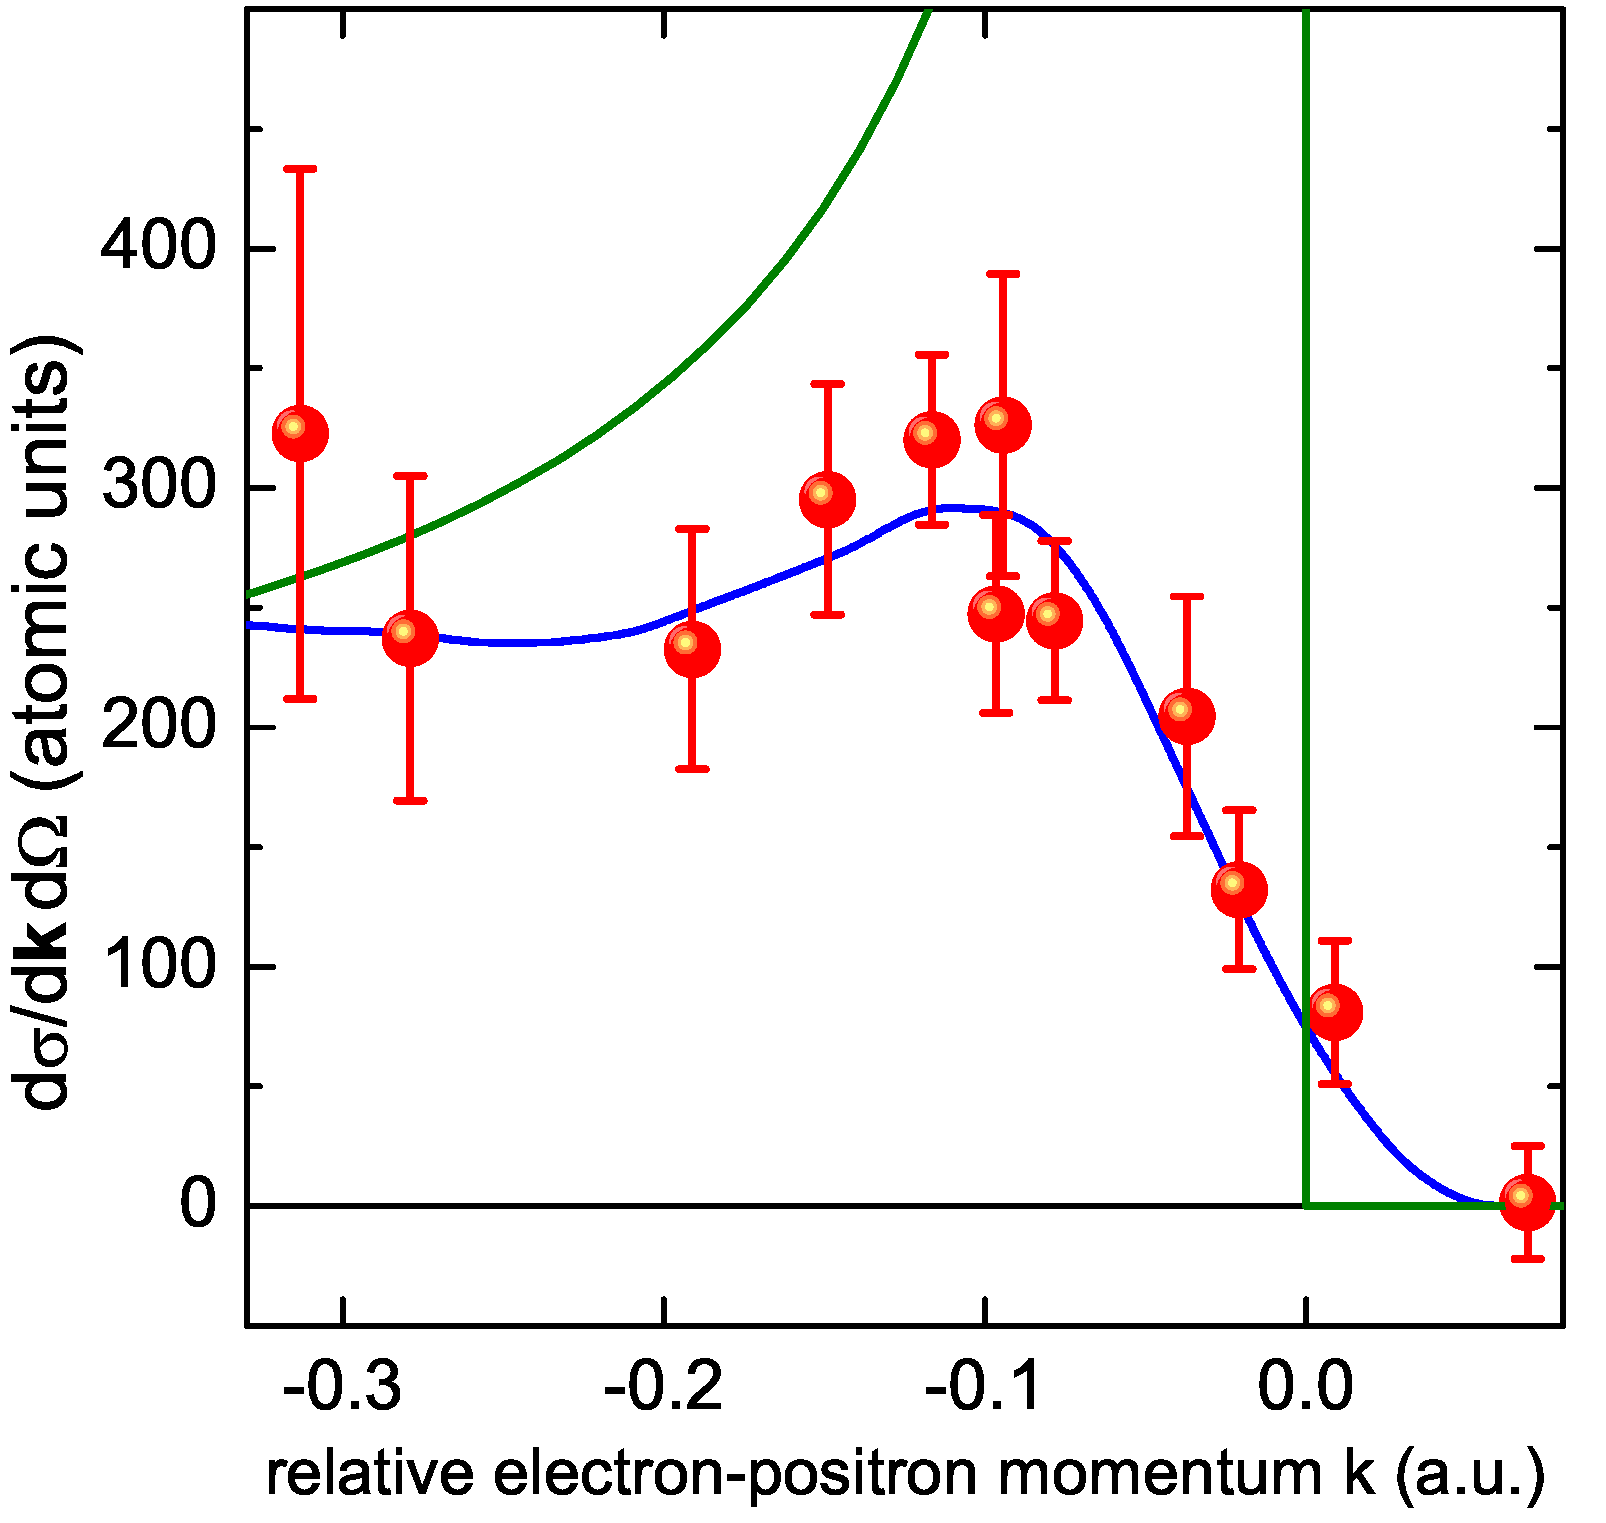
\includegraphics[width=\imsize]{ap1_f1}
\caption{Una figura con algunos puntos experimentales y curva de datos te\'{o}ricos\label{f:figura1}}  
\end{figure}



%%% Local Variables: 
%%% mode: latex
%%% TeX-master: "template"
%%% End: 



\begin{biblio}
\nocite{*}
\bibliography{referencestortoises}
\end{biblio}

%\begin{postliminary}

    %\begin{seccion}{Agradecimientos}
    
    %\end{seccion}

%\end{postliminary}

\end{document}